\section{Results}

% \begin{itemize}
%     \item Methods on how we're doing simulations and results (with simulations and experimental data)
%     \begin{itemize}
%         \item Different SNRs and maybe even use CAPs
%         \item Selection of HRF explained if both use the same but it's different from what's used for simulating.
%         \begin{itemize}
%             \item What happens? For example with gamma for simulating.
%         \end{itemize}
%         \item Selection of regularization parameter
%         \begin{itemize}
%             \item Present with real data on a voxel
%         \end{itemize}
%     \end{itemize}
% \end{itemize}

A critical decision with deconvolution methods is the selection of the regularization parameter \(\lambda\), for which many techniques have been proposed in the literature but an optimal is yet to be discovered. In fact, Paradigm Free Mapping and Total Activation base their selection of the regularization parameter on different criteria: the Bayesian Information Criterion (BIC)~\cite{schwarz1978estimating} and Akaike Information Criterion (AIC)~\cite{akaike1998information}, and a selection based on the convergence of the residuals to a pre-estimated level of the noise respectively. Hence, we compare the performance of the two algorithms with both selection criteria. Furthermore, we explore the differences between the techniques in terms of the estimation of the activity-inducing signal \(\mathbf{s}\) using the \textit{spike model} in~\eqref{eq:pfm_spike} and the innovation signal \(\mathbf{u}\) using the \textit{block model} in~\eqref{eq:pfm_block}.

\subsection{Simulated and experimental data}
\label{sec:data}

In order to compare the two methods while controlling for their correct performance, we simulated a 400 seconds (TR = 2 s) activity-inducing signal with five neuronal events, convolved it with the SPMG1 HRF, and we added noise of different sources (physiological, thermal and motion-related) with different signal-to-noise ratios (SNR = [20 dB, 10 dB, 3 dB]) that represent low, medium and high levels of noise as shown in Figure~\ref{fig:simulations}.

\begin{figure}[h]
    \begin{center}
        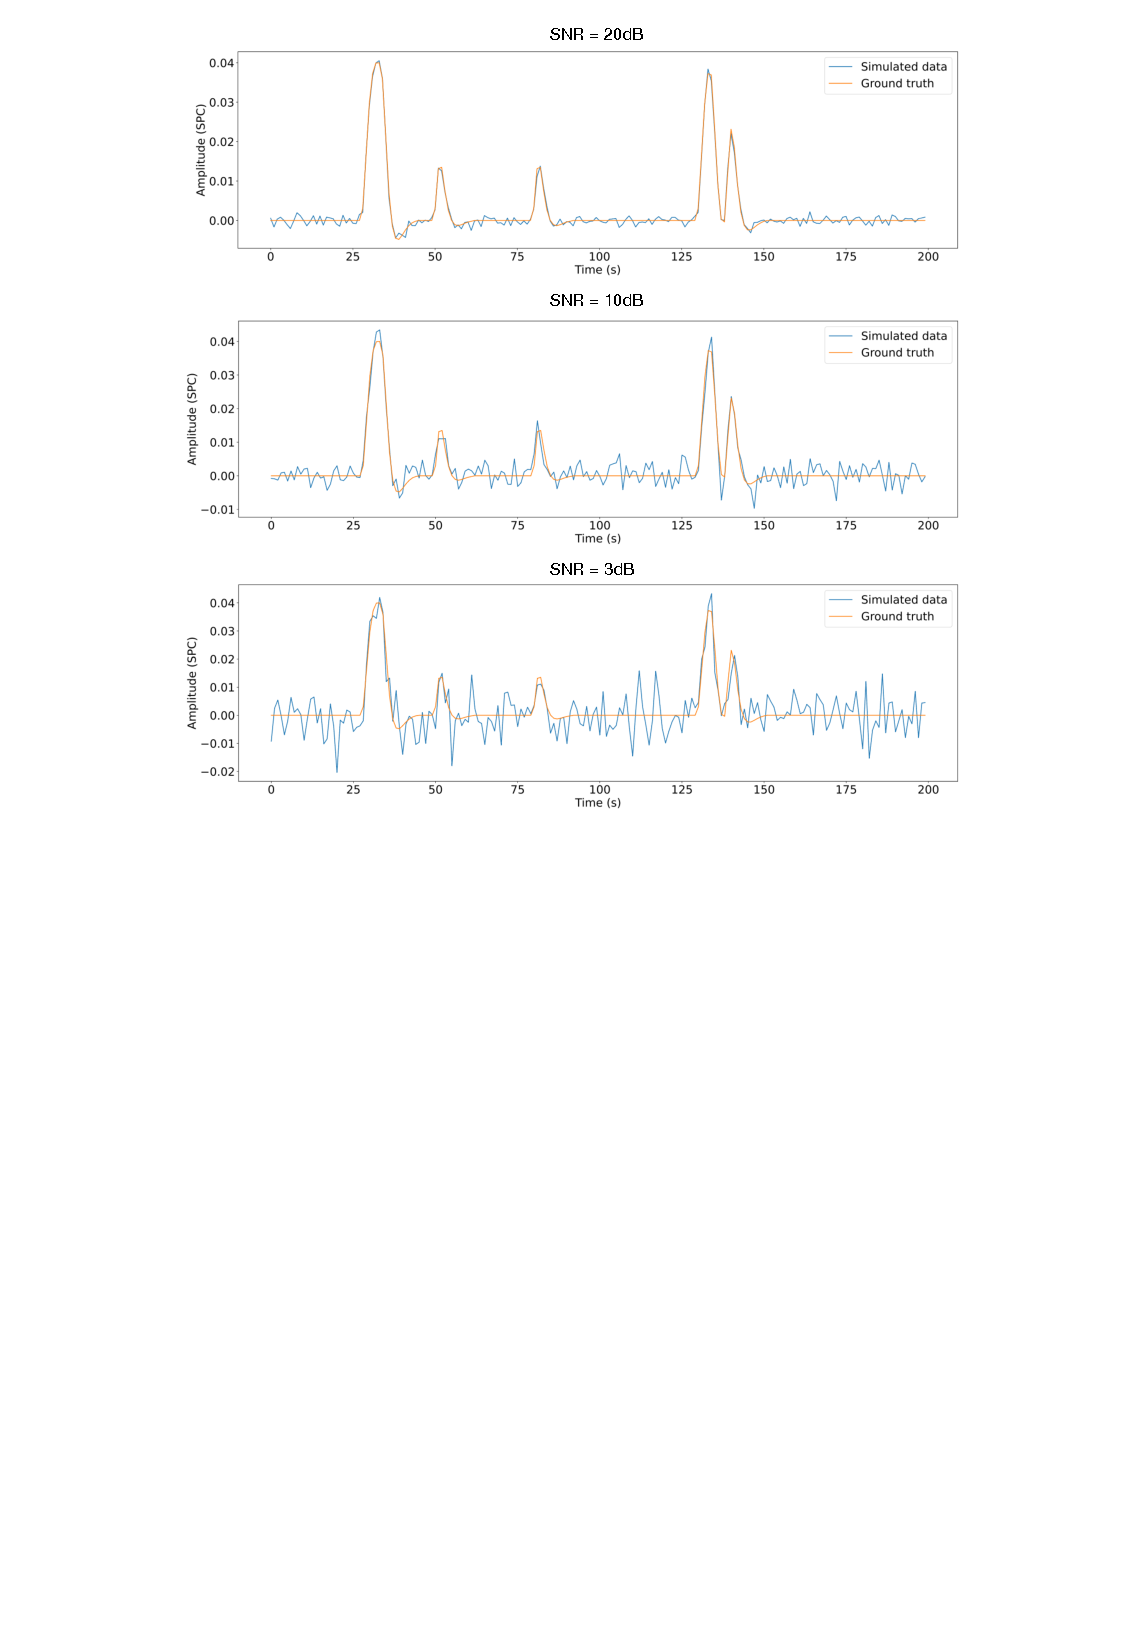
\includegraphics[width=\columnwidth]{figures/sim.pdf}
    \end{center}
    \caption{Simulated signal with different SNRs (20 dB, 10 dB and 3 dB).}
\label{fig:simulations}
\end{figure}

Furthermore, we compared the two techniques on a finger-tapping task where the ground-truth was unknown. One healthy subject was scanned in a 3T MR scanner (Siemens) as part of a larger experiment under a Basque Center on Cognition, Brain and Language Review Board-approved protocol. T2*-weighted multi-echo fMRI data was acquired with a multiband (MB) multi-echo gradient echo-planar imaging sequence (340 scans, 52 slices, Partial-Fourier=6/8, voxel size=2.4x2.4x3 mm\textsuperscript{3}, TR=1.5 s, TEs=10.6/28.69/46.78/64.87/82.96 ms, flip angle=70\(^o\), MB factor=4, GRAPPA=2). During the fMRI acquisition, subjects performed a motor task consisting of five different movements (left-hand finger tapping, right-hand finger tapping, moving the left toes, moving the right toes and moving the tongue). These conditions were randomly intermixed every 16 seconds, and were only repeated once the entire set of stimuli were presented. Data preprocessing consisted of optimally combining the echo time datasets, detrending of up to 5\(^{th}\)-order Legendre polynomials, spatial smoothing (3 mm FWHM) and normalization to signal percentage change. For this comparison, we selected a voxel that best represented the right-hand finger-tapping paradigm as shown in Figure~\ref{fig:finger_tapping}.

\begin{figure}[h]
    \begin{center}
        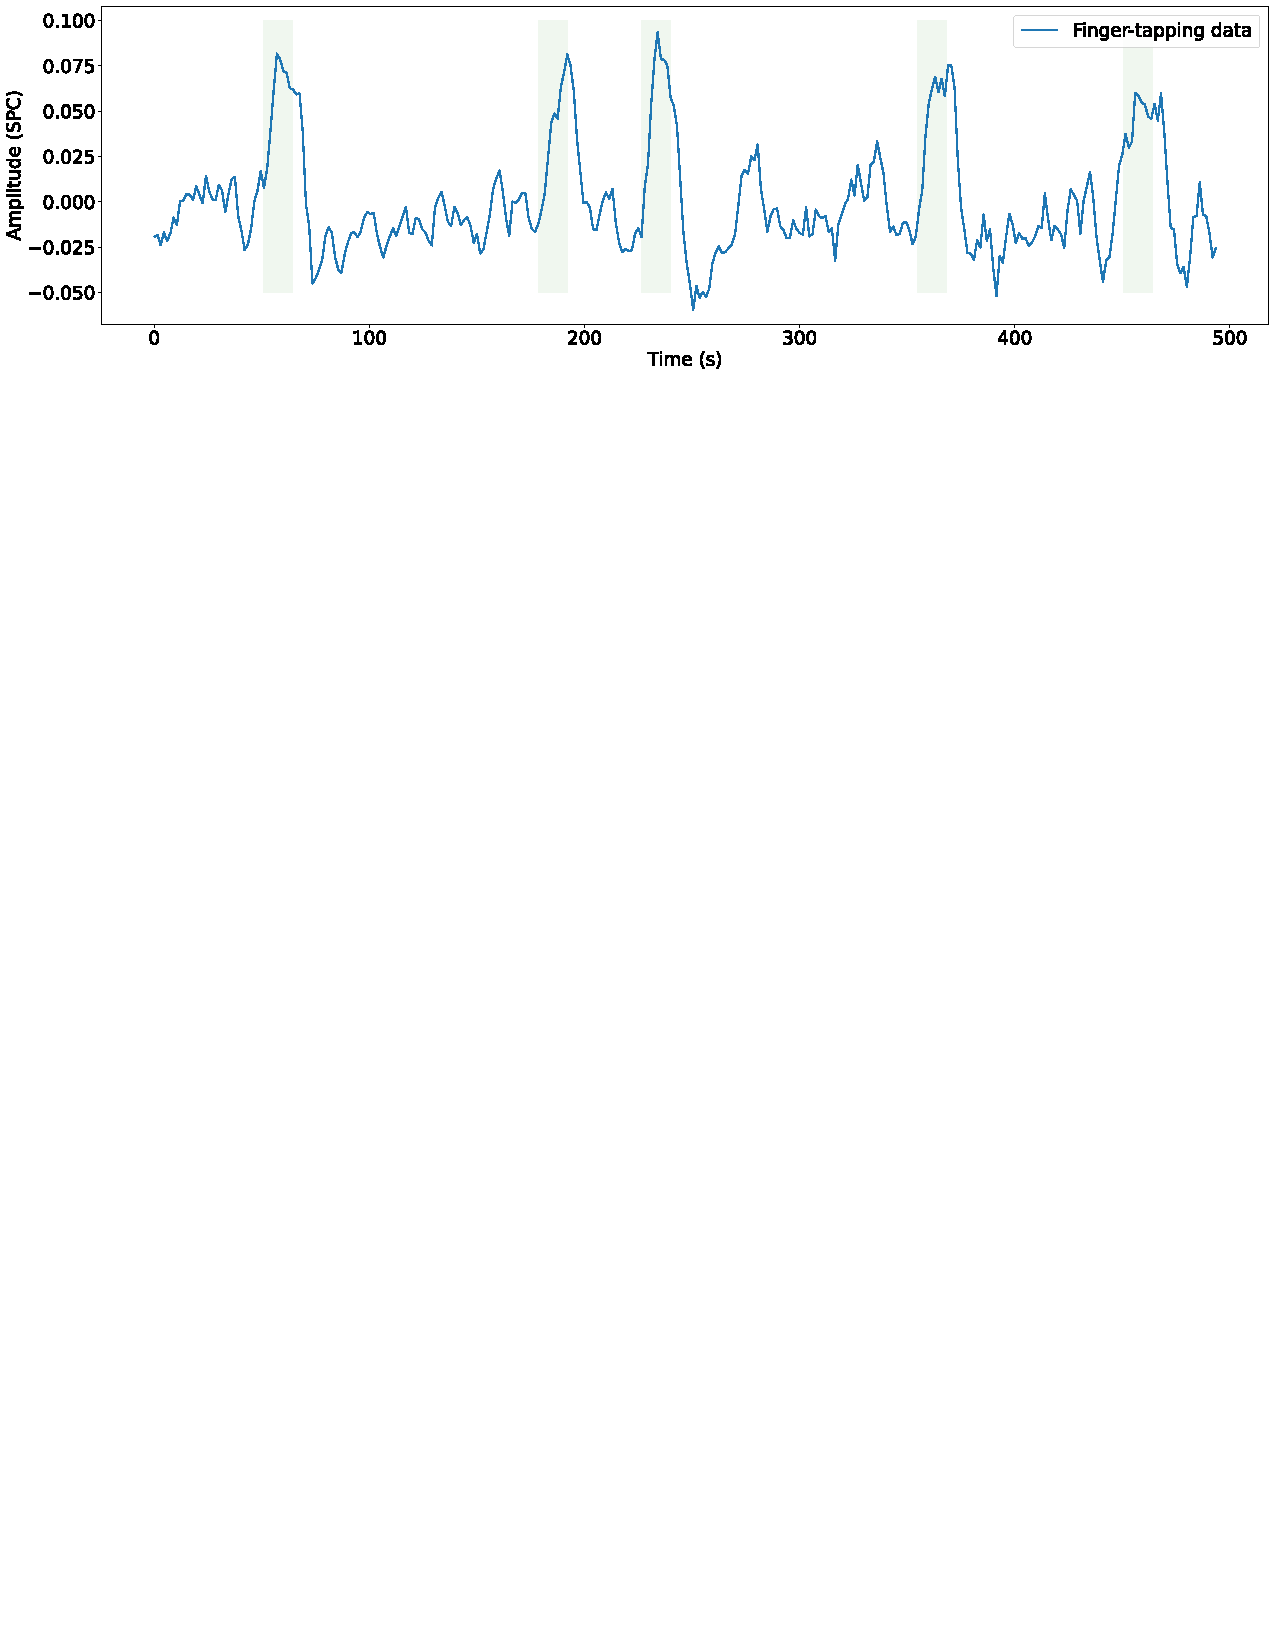
\includegraphics[width=\columnwidth]{figures/finger_tapping.pdf}
    \end{center}
    \caption{Most representative voxel of the finger-tapping task. Green blocks indicate the onsets and the duration of it.}
\label{fig:finger_tapping}
\end{figure}

\subsection{Selection of the hemodynamic response function}

\begin{figure}[h]
    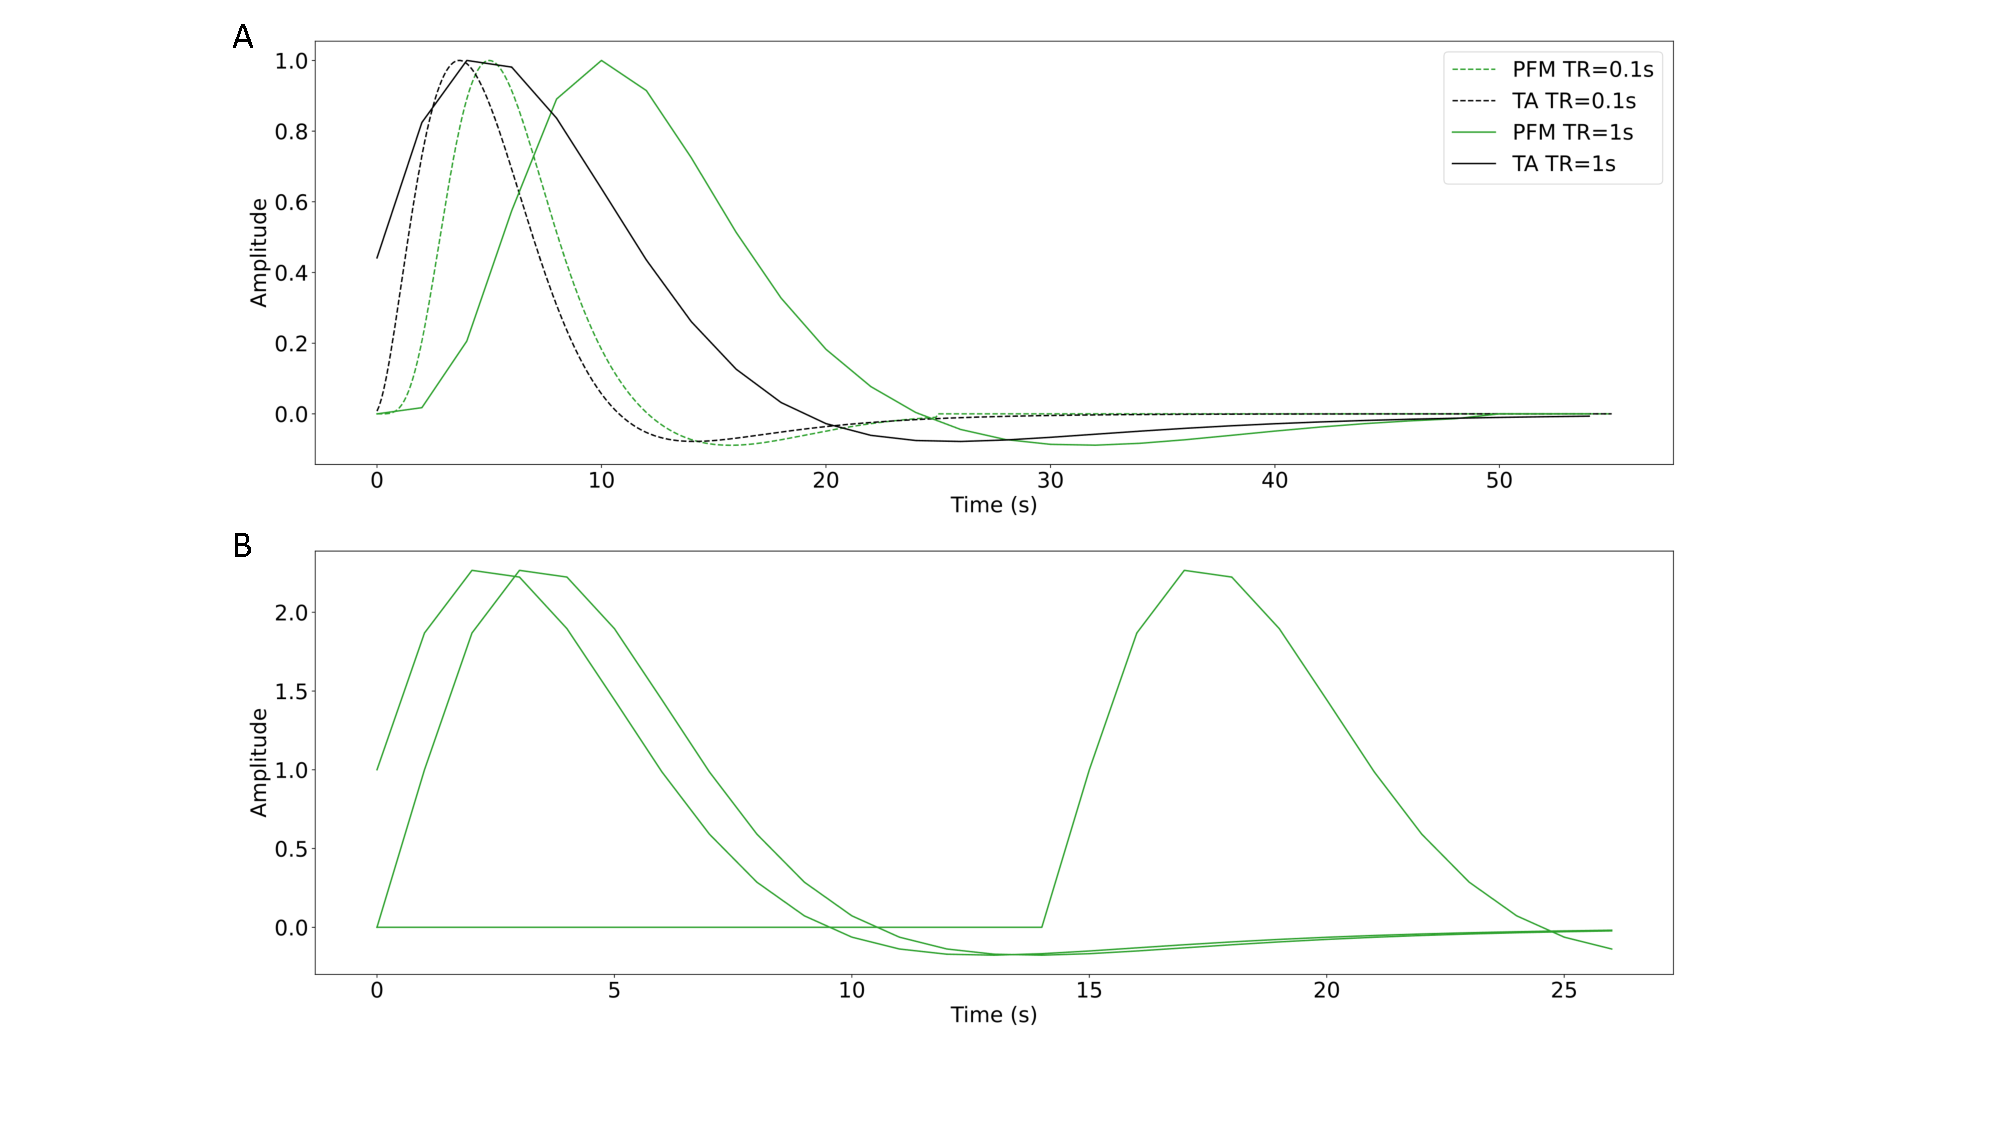
\includegraphics[width=\columnwidth]{figures/pfm_ta_hrf.pdf}
    \caption{A) Canonical HRF models typically used by PFM (green) and TA (black) at TR = 0.1 s (dashed lines) and TR = 1 s (solid lines). Without loss of generality, the waveforms are scaled to unit amplitude for visualization. B) Representation of three shifted HRFs at TR=1 s (onsets=0, 1, and 15 s) that build the design matrix for PFM when the HRF model has been matched to that in TA.}
\label{fig:hrf_diff}
\end{figure}

With the aim of making a fair comparison of the two methods, we first compared their hemodynamic response functions. Figure~\ref{fig:hrf_diff}A shows the difference in the hemodynamic response function that PFM and TA use by default for TR = 0.1 s and TR = 1 s adjusted to a peak amplitude of one; i.e. the SPMG1 and the HRF resulting from the linear differential operator. The most observable difference between the two HRF is the time to peak: the HRF used by Total Activation does not begin at zero while the one used by PFM does.

While Paradigm Free Mapping allows for the use of any hemodynamic response function --- the columns of the design matrix \(\mathbf{H}\) are composed by shifted versions of the HRF--- the linear differential operator in TA is tailored for a fixed HRF. Hence, for practical reasons, we reproduced the HRF in the Total Activation filter and incorporated it into the PFM formulation (Figure~\ref{fig:hrf_diff}B).

\subsection{Selection of the regularization parameter based on the estimation of the noise}

\begin{figure*}[t!]
    \begin{center}
        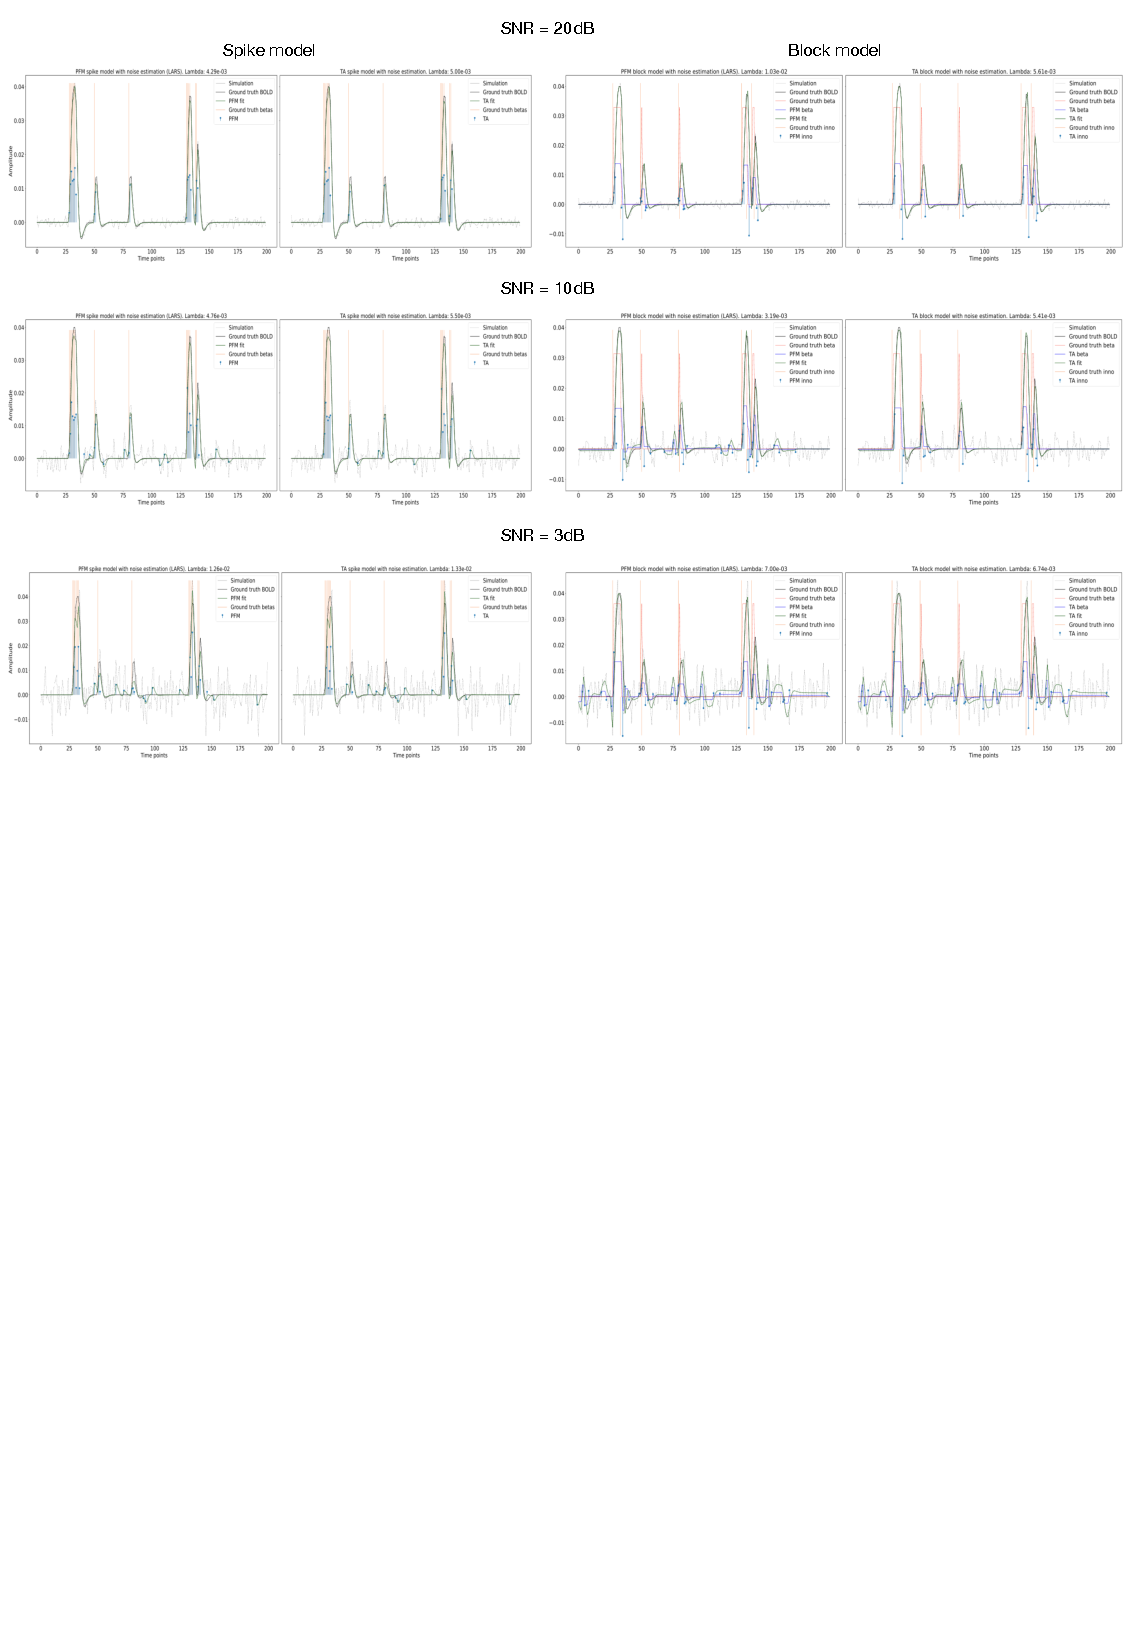
\includegraphics[width=\textwidth]{figures/std_based.pdf}
    \end{center}
    \caption{Estimated activity-inducing, innovation and activity-related (fit, \(\mathbf{x}\)) signals when \(\lambda\) is selected based on convergence of residuals to have same variance as MAD estimate of noise with spike model (left, with PFM on the left and TA on the right) and block model (right, with PFM on the left and TA on the right) on SNR = 20dB (top), SNR = 10dB (middle) and SNR = 3dB (bottom).}
\label{fig:std}
\end{figure*}

\begin{figure*}[t!]
    \begin{center}
        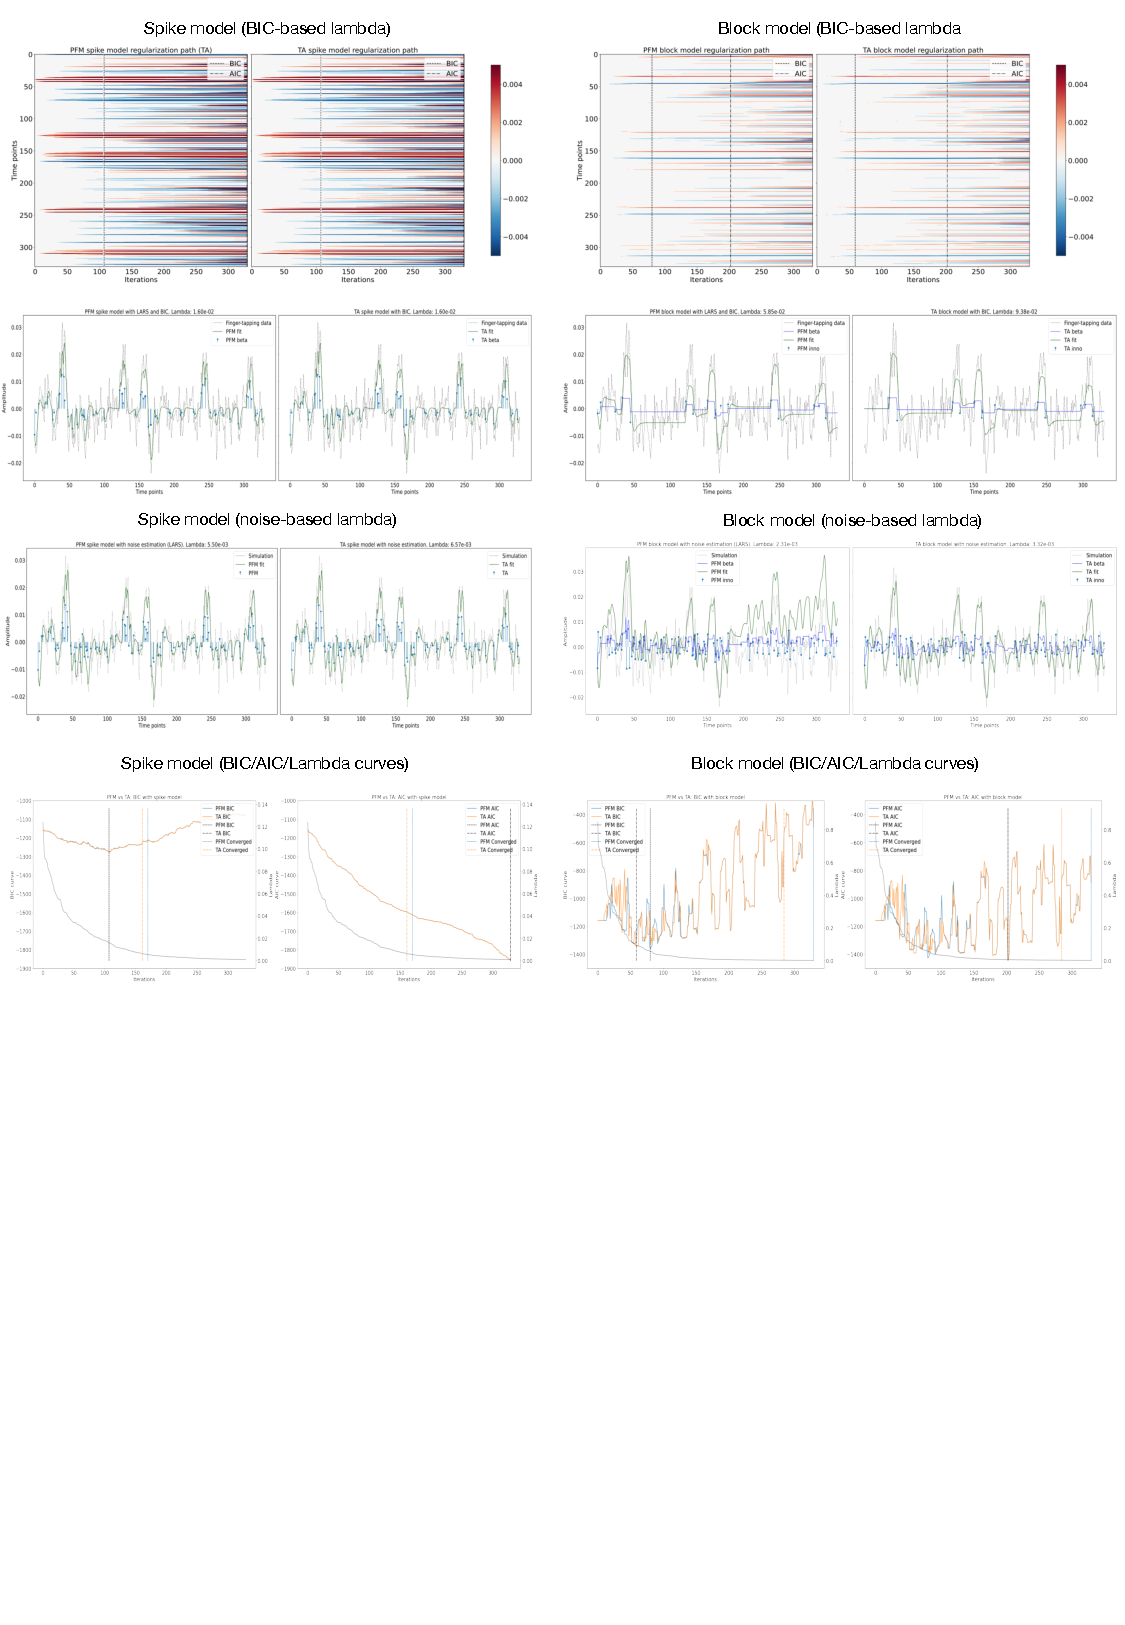
\includegraphics[width=\textwidth]{figures/exp.pdf}
    \end{center}
    \caption{(Row 1) Regularization paths of the estimated activity-inducing signal (spike model --- left) and innovation signal (block model --- right); (Row 2) activity-inducing, innovation and activity-related (fit, \(\mathbf{x}\)) signals when \(\lambda\) is selected based on BIC, or (Row 3) based on convergence of residuals to have same variance as MAD estimate of noise; (Row 4) Corresponding curves of BIC and AIC, where the vertical lines indicate the three options to select \(\lambda\) (BIC, AIC and Converged/MAD).}
\label{fig:exp}
\end{figure*}

Total Activation proposes to solve the inverse problem by updating the regularization parameter \(\lambda\) on every iteration \(n\) so that the residuals converge to a previously estimated noise level of the data fit \(\tilde{\sigma}\), where this pre-estimated noise is calculated from the median absolute deviation of fine-scale wavelet coefficients (Daubechies, order 3)~\cite{karahanouglu2013total}:

\begin{equation}
    \lambda^{n+1} = \frac{N \tilde{\sigma}}{\frac{1}{2} \| \mathbf{y} - \mathbf{x}^n \|_F^2} \lambda^n.
\label{eq:std}
\end{equation}

Thus, we calculated the regularization path with PFM (as described in \ref{sec:regpath}) and selected the \(\lambda\) corresponding to the residuals that were closest to the estimated noise level of the data. We applied Total Activation with temporal regularization in its original form. Figure~\ref{fig:std} depicts the estimated activity-inducing, innovation and activity-related signals when updating \(\lambda\) as in~\eqref{eq:std} in the three simulated SNR settings using the spike model (left) and the block model (right). Figure~\ref{fig:std} (left) shows nearly identical results between PFM (left) and TA (right). The minimal differences are the result of slight dissimilarities in the convergence of the residuals to the estimated noise level of the data. Likewise, the use of the block model with a selection of \(\lambda\) based on the convergence of the residuals to have the same variances as the MAD estimate of the noise yields results that are identical in practice as shown in Figure~\ref{fig:std} (right).

In addition, we performed the same comparison on experimental data as introduced in~\ref{sec:data}. Figure~\ref{fig:exp} (row 3) illustrates that the estimated activity-inducing, innovation and activity-related signals with PFM and TA are once again practically identical both for the spike model (left) and the block model (right).

\subsection{Selection of the regularization parameter by solving the regularization path}
\label{sec:regpath}

\begin{figure*}[t!]
    \begin{center}
        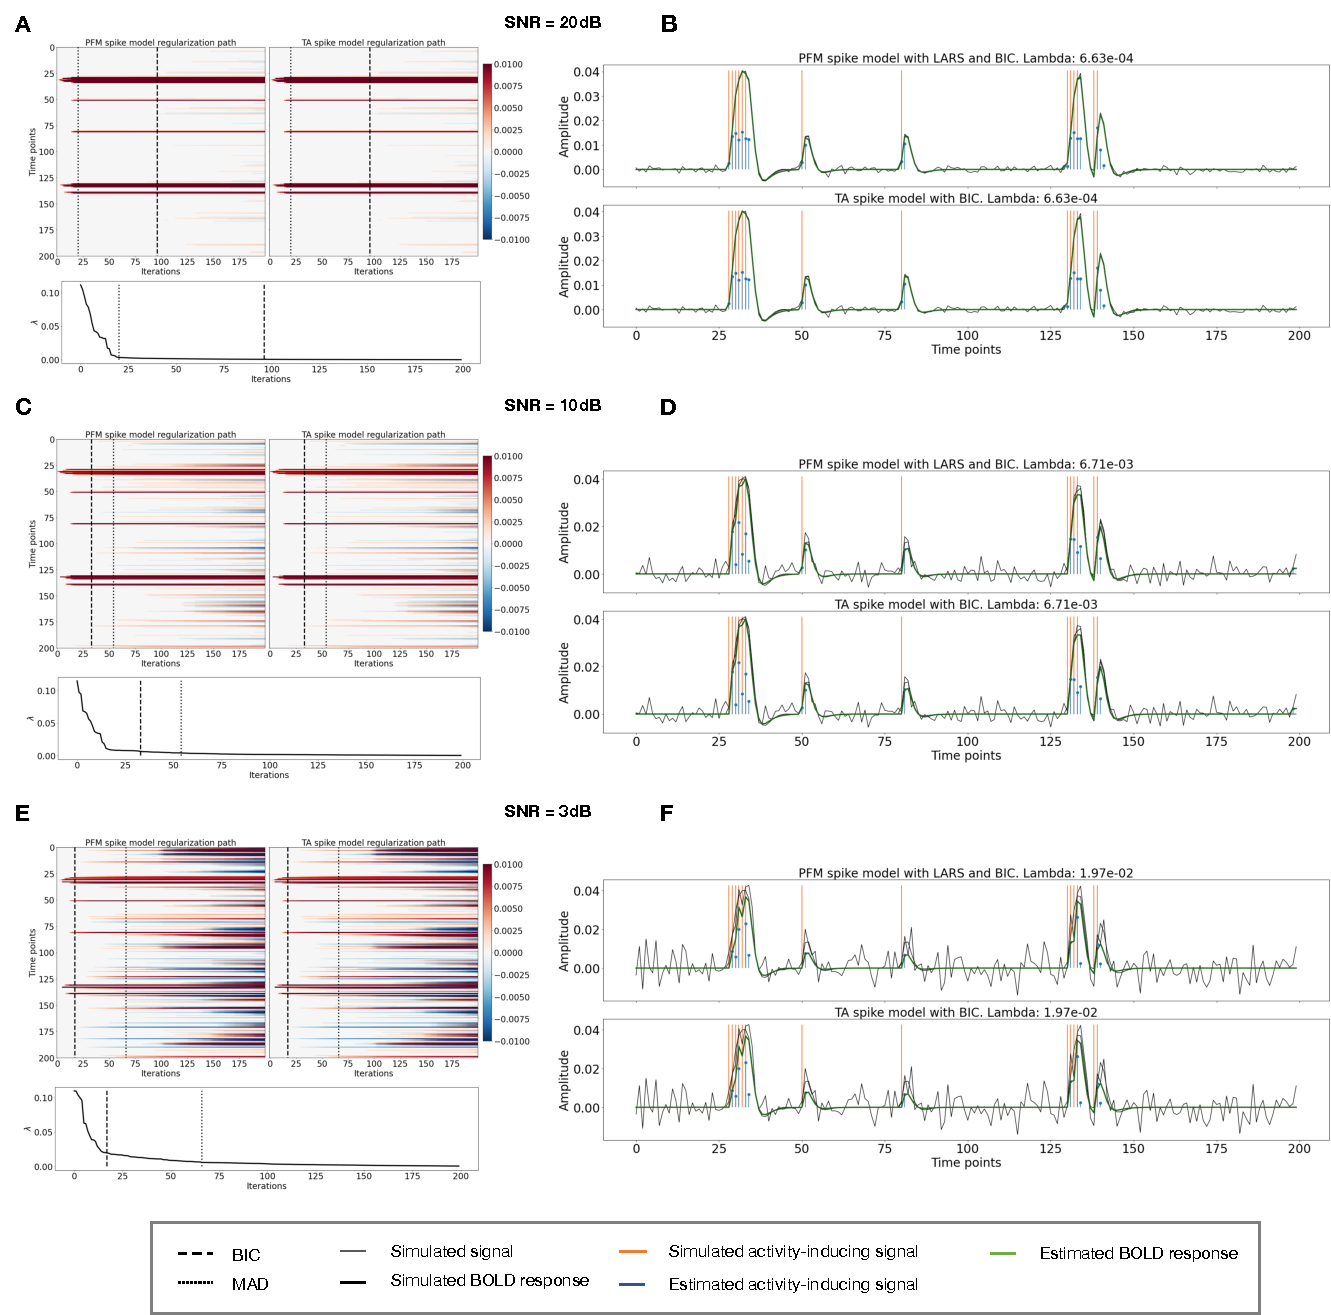
\includegraphics[width=\textwidth]{figures/regpath_spike.pdf}
    \end{center}
    \caption{Spike model simulations. (Left) Heatmap of the regularization paths of the activity-inducing signal estimated with PFM and TA as a function of (increasing number of iterations in x-axis), whereas each row in the y-axis shows one time-point. Vertical lines denote iterations corresponding to the Akaike and Bayesian Information Criteria (AIC and BIC). (Right) Estimated activity-inducing (blue) and activity-related (green) signals when is set based on BIC. All estimates of are identical, regardless of SNR.}
\label{fig:path_spike}
\end{figure*}

\begin{figure*}[t!]
    \begin{center}
        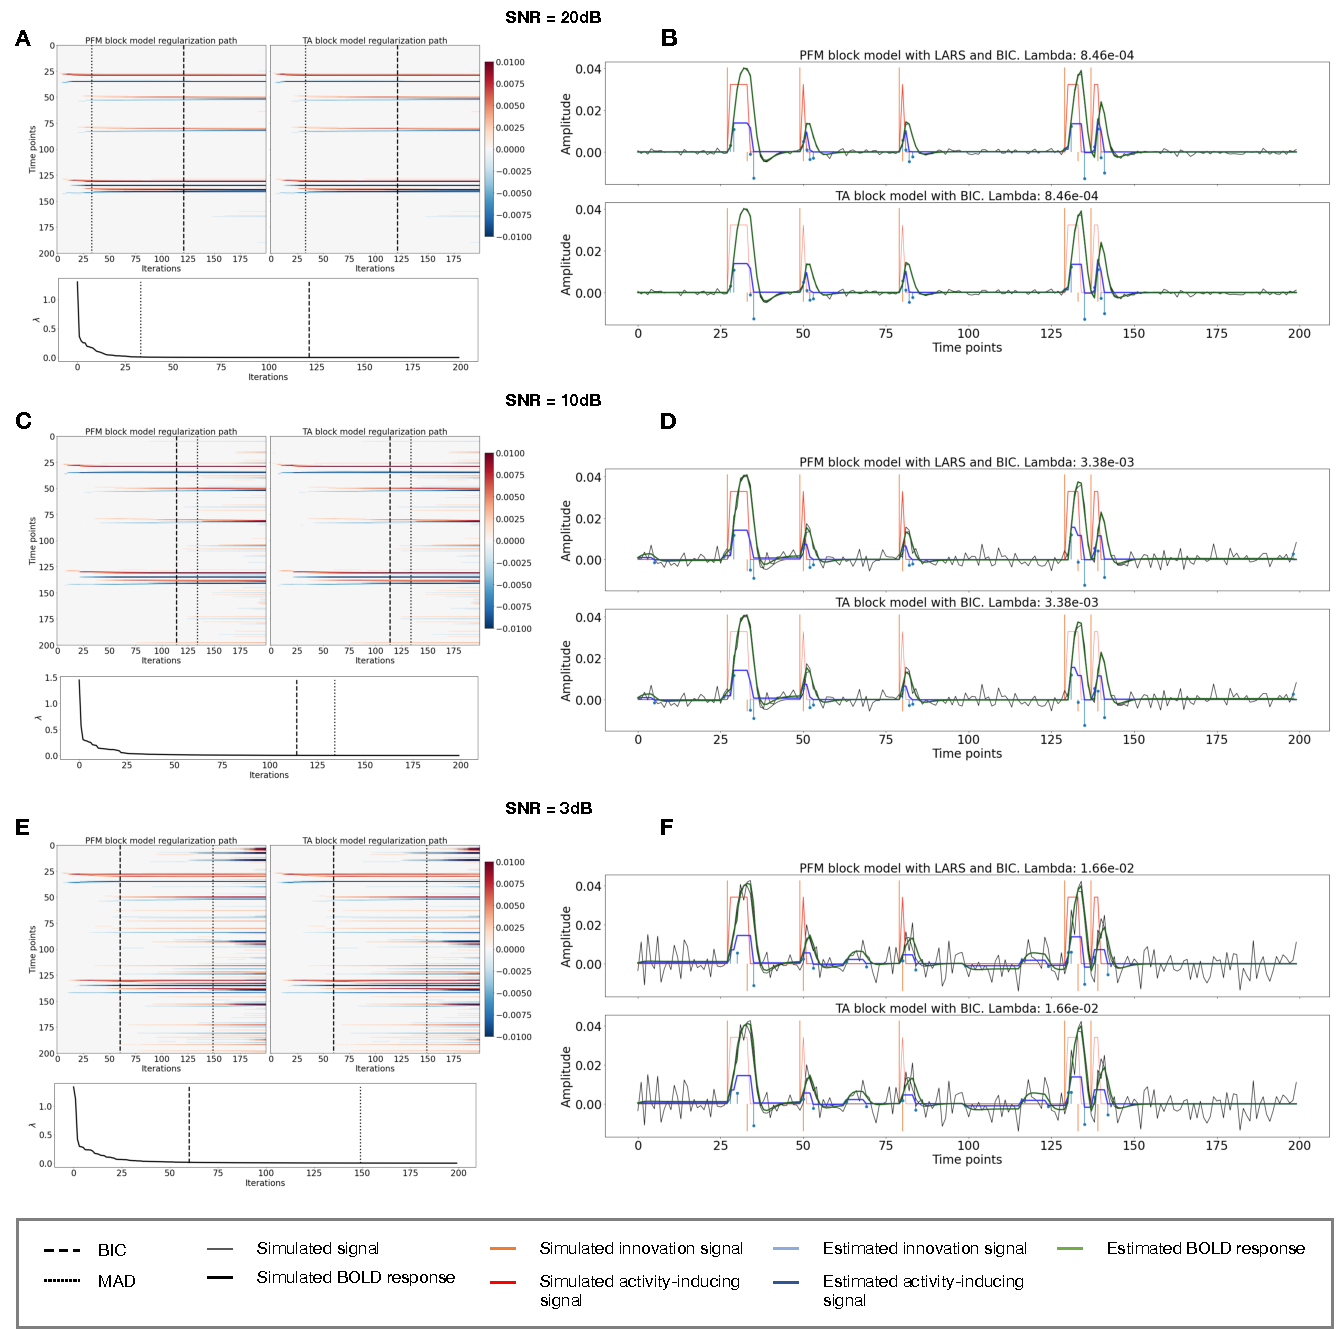
\includegraphics[width=\textwidth]{figures/regpath_block.pdf}
    \end{center}
    \caption{Block model simulations. (Left) Heatmap of the regularization paths of the innovation signal estimated with PFM and TA as a function of (increasing number of iterations in x-axis), whereas each row in the y-axis illustrates one time-point. Vertical lines denote iterations corresponding to the Akaike and Bayesian Information Criteria (AIC and BIC). (Right) Estimated innovation (blue) and activity-related (green) signals when is set based on BIC. All the estimates of are identical, regardless of SNR.}
\label{fig:path_block}
\end{figure*}

\begin{figure*}[t!]
    \begin{center}
        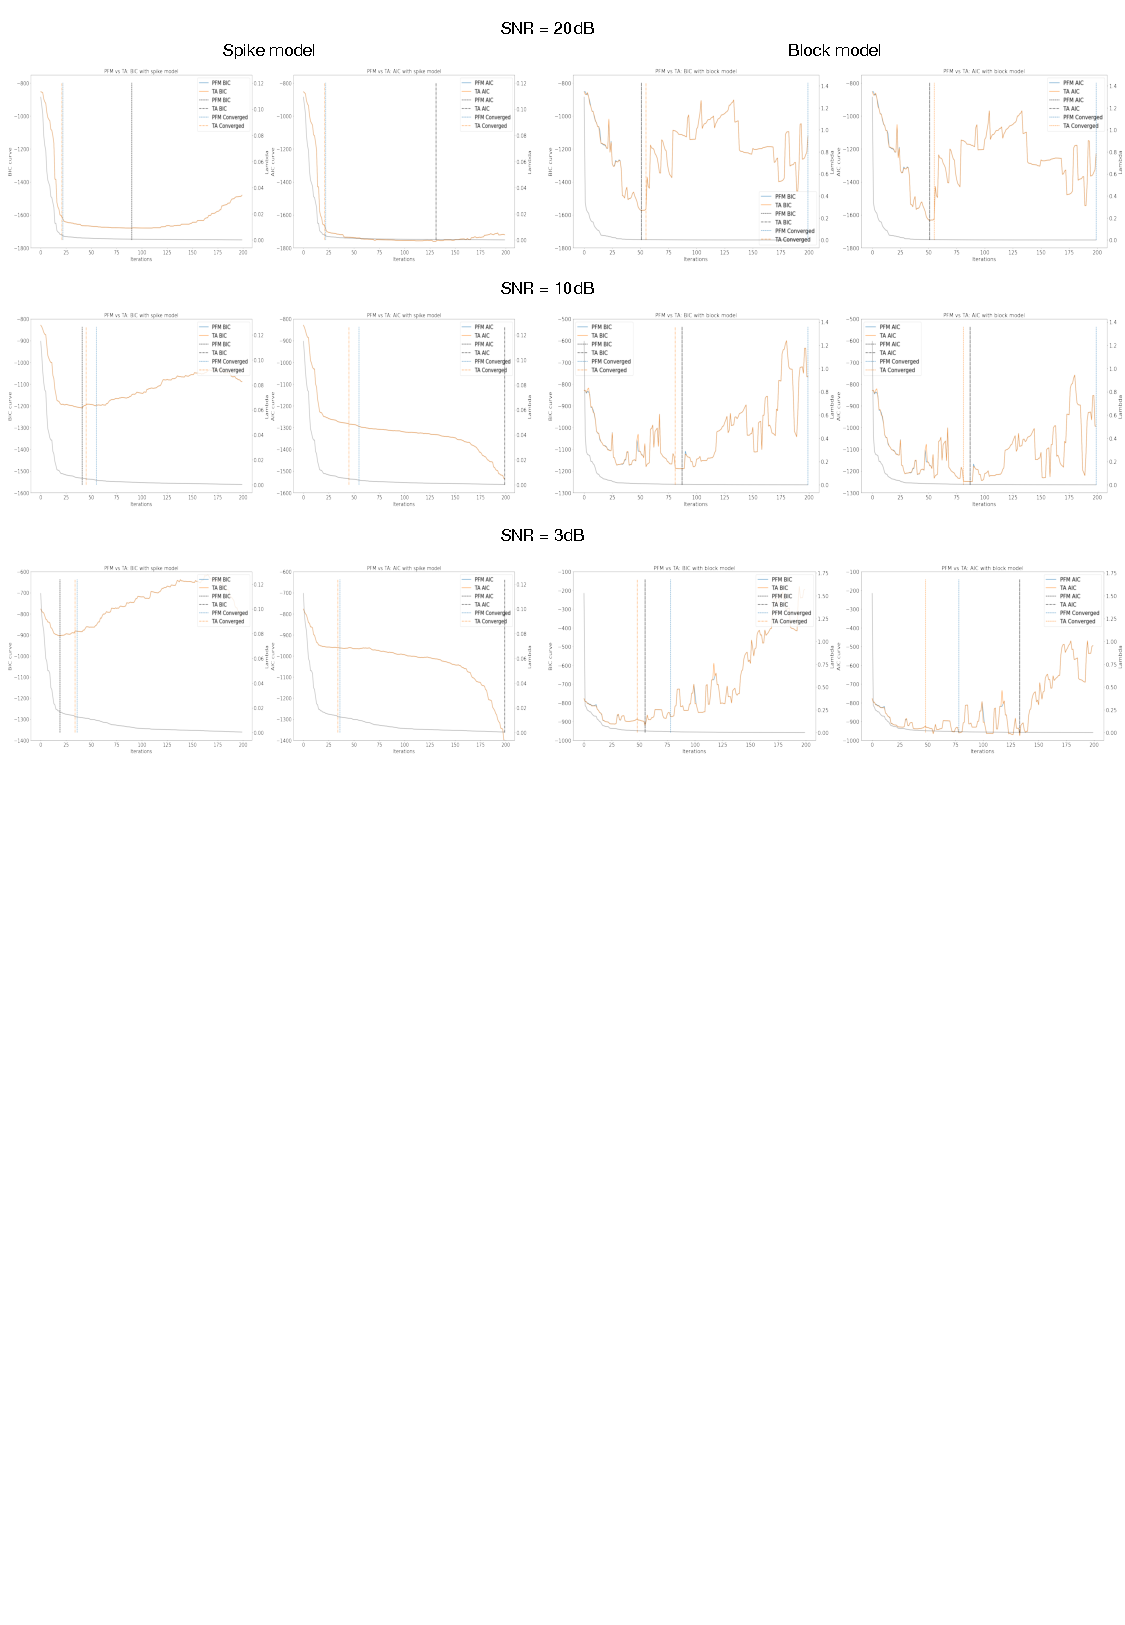
\includegraphics[width=\textwidth]{figures/lambda_cost.pdf}
    \end{center}
    \caption{Lambdas and cost.}
\label{fig:lambdas}
\end{figure*}

Paradigm Free Mapping bases its selection of the regularization parameter on the Bayesian Information Criterion (BIC)~\cite{schwarz1978estimating} and the Akaike Information Criterion (AIC)~\cite{akaike1998information}. Hence, we calculated the regularization path with PFM by means of the least angle regression (LARS) algorithm~\cite{efron2004least} and used the \(\lambda\) in the path to solve the deconvolution problem with Total Activation.

Figure~\ref{fig:path_spike} (left) shows the regularization path of PFM and TA side by side for the three SNR conditions for the spike model; i.e., the inverse problem described in~\eqref{eq:pfm_spike}. Each iteration of LARS reduces the value of \(\lambda\); i.e., reduces the sparsity promoted by the \(l_1\)-norm, and reveals a new non-zero coefficient as shown in the x axis of the heatmaps. Vertical black lines depict the selection of the regularization parameter based on BIC and AIC, and thus, the colored coefficients to the left of the vertical lines depict the estimated activity-inducing signal \(s(t)\). Figure~\ref{fig:path_spike} (right) illustrates the resulting estimation of the activity-inducing and neuronal-related signals when basing the selection of \(\lambda\) on BIC for the three simulated SNR conditions. Given that the regularization paths of both techniques are identical, the BIC-based selection of the regularization parameter and the results of deconvolving with said \(\lambda\) are identical too (see Figure~\ref{fig:lambdas}). Thus, Figure~\ref{fig:path_spike} demonstrates that, regardless of the simulated SNR condition, both deconvolution algorithms produce identical regularization paths when the same HRF and regularization parameters are applied, and hence, identical estimates of the activity-inducing signal \(\mathbf{s}\) and neuronal-related signal \(\mathbf{x}\).

The regularization path to estimate innovation signals; i.e., solving the optimization problem using the block model in~\eqref{eq:pfm_block}, yields mainly undistinguishable results for both PFM and TA methods as shown in Figure~\ref{fig:path_block} (left). Again, the BIC-based selection of \(\lambda\) is identical for both PFM and TA and the estimation of the innovation signal \(\mathbf{u}\) shows no distinguishable differences between the algorithms (see Figure~\ref{fig:path_block} right). Figure~\ref{fig:lambdas} (right) demonstrates that the  Therefore, both Paradigm Free Mapping and Total Activation yield nearly-identical regularization paths and estimates of the innovation signal regardless of the simulated SNR condition when applying the same HRF and regularization parameters with the block model.

Furthermore, we performed the same analysis on experimental data as shown in Figure~\ref{fig:exp} (rows 1-2, 4). Row 1 demonstrates that the PFM and TA regularization paths are identical when deconvolving experimental data, regardless of the deconvolution model (spike or block). Even though tiny differences can be seen between the two methods in the BIC and AIC selection of \(\lambda\) in row 4, row 2 
